\documentclass[12pt]{article}
\usepackage{geometry}
\geometry{letterpaper, left=22.5mm, right=22.5mm, top=30mm, bottom=30mm}
\geometry{letterpaper}
\usepackage{amsmath}
\usepackage{amssymb}
\usepackage{enumitem}
\usepackage{fancyhdr}
\usepackage{framed}
\usepackage{tikz}
\usepackage{mathpazo}
%\usepackage{charter}
%\usepackage{newcent}
\usepackage{indentfirst}
\usepackage{booktabs}
\usepackage{graphicx}
\usepackage{float}
\usepackage{makecell}
\usepackage{xcolor}
\usepackage{mdframed}
\usetikzlibrary{trees}
\pagestyle{fancy}
\usepackage{amsthm}
\theoremstyle{definition}
\newtheorem{definition}{Definition}[section]
\theoremstyle{property}
\newtheorem{property}{Property}[section]
\theoremstyle{assumption}
\newtheorem{assumption}{Assumption}[section]
\theoremstyle{example}
\newtheorem{example}{Example}[section]
\theoremstyle{comment}
\newtheorem{comment}{Comment}[section]
\newtheorem{theorem}{Theorem}[section]
\newtheorem{corollary}{Corollary}[theorem]
\newtheorem{lemma}[theorem]{Lemma}
\usepackage{lastpage}
\usepackage{wrapfig}
\usepackage{hyperref}
\usepackage{subcaption}
\usepackage{setspace}
\hypersetup{
colorlinks=true,
linkcolor=black,
filecolor=green, 
urlcolor=blue,
}
\newcommand{\ROM}[1]
    {\MakeUppercase{\romannumeral #1}}
\fancyhead[L]{Econometrics \ROM{2}: Recitation 12 }%change each reci
\fancyhead[R]{Spring 2020}
\fancyfoot[C]{\thepage \hspace{1pt} / \pageref{LastPage}}

\fancypagestyle{firstpage}{%
\fancyhf{}%
\renewcommand{\headrulewidth}{0mm}%
  \fancyfoot[C]{\thepage \hspace{1pt} / \pageref{LastPage}}
}
%change title each rec
\title{Introduction to Econometrics \ROM{2}: Recitation 12\footnote{This is based on the lecture notes of Professors Jushan Bai and Bernard Salanie. I was also greatly helped by previous recitation notes from Paul Sungwook Koh and Dong Woo Hahm. The remaining errors are mine. }}

\begin{document}
\linespread{1.25}
\onehalfspacing

\author{Seung-hun Lee\footnote{Contact me at \href{mailto:sl4436@columbia.edu}{sl4436@columbia.edu} if you spot any errors or have suggestions on improving this note.}}
\date{April 29th, 2020}
\maketitle
\thispagestyle{firstpage}

%%%%%%%%%%%%%%%%%%
\section{Regression Discontinuity}

\textbf{Regression discontinuity} (commonly abbreviated to RD or RDD) approach actually started from Psychology in 1960s and was brought into the mainstream of applied economics very recently. Whenever you learn applied microeconomics class in your second year, you are bound to read or present about a paper that uses this research design. \par
As its name suggests, this approach exploits the discontinuities in the treatment assignment. So the key difference between regression discontinuity and previous frameworks is that RDD does not require the overlap condition in the sense that $p(X_i)\in(0,1)$. In fact, one of the design has $p(X_i)=1$ for $X_i\geq c$ and $0$ otherwise. Another thing that RDD should satisfy is that for every other covariates, the distribution should remain continuous even through the discontinuity.\par
This is usually presented visually through graphs - one with the covariate that determines assignment to the treatment, usually called the forcing (running) variable $W_i$ and the treatment status $D_i$, the other with the $W_i$ and all other covariates $X_i$. For instance, if we are in the public finance context and study the effect of a particular welfare program with a means-tested benefit assignment mechanism, we could use the means-tested criteria as our $W_i$. If we are to study the effect of a specific educational program offered to those below a particular test score, that score could be the $W_i$. Here are some works that deal use RDD. 


\begin{mdframed}[backgroundcolor=yellow!5] 
\begin{example}[Lee, 2007] This paper focuses on the elections won and lost by a very narrow margin. The logic is that in such case, winning and losing is effectively randomized. The running variable is the Democrat vote share $-$ Republican vote share, or a margin of victory/loss. One of the findings is that Democrats who barely win an election are much more likely to run for office and succeed in the next election, compared to Democrats who barely lose. In general this paper finds positive relationship between margin of victory and electoral outcomes, both in terms of vote shares and wins by individuals and parties. 
\end{example}


\begin{example}[Howell, 2017] This paper assess the impact of R\&D subsidies from the government to new ventures. The rank on the application to the R\&D is used as a running variable, (and this is a sharp RDD and a discrete running variable\footnote{Because of the discreteness, McCrary test is infeasible.}).  The paper finds that an early-stage award approximately doubles the probability that a firm receives subsequent venture capital (summarized in the figure below) and has large, positive impacts on patenting and revenue. These effects are stronger for more financially constrained firms.
\end{example}
\begin{figure}[H]
\centering
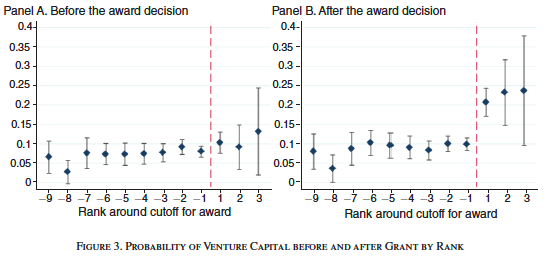
\includegraphics[width=0.7\textwidth, keepaspectratio]{RD_fig.png}
\caption{Reception of venture capital, before and after}
\end{figure}
\begin{example}[Ost, Pan \& Weber, 2018] This paper estimates the return to college using admin data on college enrollment and earnings from Ohio. The running variable here is a GPA, in that this paper uses the fact that colleges dismiss low-performing students on certain GPAs. RDD is used to measure effects of college on earnings. This paper finds that dismissal leads to a short-run increase in earnings and tuition savings, which are wiped out by gains from college graduates 8 years after. They also carry out the test that the result is not driven by manipulation.
\end{example}
\end{mdframed}


\subsection{Framework}
We will start with a \textbf{sharp RDD}. You can think of this case as a case where the assignment into the treatment is determined by
\[
D_i=1(W_i\geq c(X_i))
\]
where $c(X_i)$ can be a known function of $X_i$ or just a constant. We also keep the potential outcome framework from before, but we will slightly change this to
\begin{align*}
Y_i& = D_iY_i(1)+(1-D_i)Y_i(0)\\
&=Y_i(0)+D_i(Y_i(1)-Y_i(0))\\
&=Y_i(0)+1(W_i\geq c(X_i))\cdot(Y_i(1)-Y_i(0))
\end{align*}
We also keep the regressional framework for the potential outcomes, $Y_i(d)=\mu(X_i,W_i,d)+\epsilon_i(d)$. So we have
\[
E[Y_i(d)|X_i,W_i]=\mu(X_i.W_i.d)
\]
One key assumption that we will carry through this section is the continuity of the conditional expectation on potential outcomes at $W_i=c(X_i)$
\begin{mdframed}[backgroundcolor=blue!5] 
\begin{assumption}[Continuity of $\mu(X_i,W_i,d)$ at $W_i=c$] If $W_i$ has a known cutoff at $c$, we assume that $E[Y_i(1)|X_i, W_i]$ and $E[Y_i(0)|X_i, W_i]$ are continuous around $W_i=c$. Put if differently, 
\[
E[Y_i(d)|X_i, W_i=c^+]=E[Y_i(d)|X_i, W_i=c^-] \ \text{for each } d\in\{0,1\}
\]
\end{assumption}
\end{mdframed}
The above condition also implies that $(\epsilon_i(1), \epsilon_i(0))$ also has a continuous distribution around $W_i=c(X_i)$. If this condition is not satisfied, this implies that there could be more than the $W_i$ variable that jumps around the cutoff, which is what you do not want in an RDD regression.  \par
There is another version of the RDD which is more general than the sharp RDD. A \textbf{fuzzy RDD} setup exploits the jump in the probability of being treated at $W_i=c$. This jump is not necessarily from 0 to 1. Formally, we say we look for discontinuities of 
\[
\Pr(D_i|X_i,W_i)
\]
at $W_i=c(X_i)$. 
\subsection{Identification in RDD}
We start with a sharp RDD case. Assume that $c(X_i)$ is a constant $c$. We can write
\begin{align*}
E[Y_i|X_i, W_i]&=E[Y_i(0)|X_i, W_i]+E[(Y_i(1)-Y_i(0))1(W_i\geq c(X_i))|X_i, W_i]
\end{align*}
And we can separate the above into two. One with $W_i=c^+$ and the other with $W_i=c^-$.
\begin{align*}
E[Y_i|X_i, W_i=c^+]&=E[Y_i(0)|X_i, W_i=c^+]+E[(Y_i(1)-Y_i(0))|X_i, W_i=c^+]\\
E[Y_i|X_i, W_i=c^-]&=E[Y_i(0)|X_i, W_i=c^-]
\end{align*}
This is because $1(W_i\geq c(X_i))=1$ if $W_i=c^+$ and 0 otherwise. Therefore, 
\begin{align*}
E[Y_i|X_i, W_i=c^+] - E[Y_i|X_i, W_i=c^-]&=E[Y_i(0)|X_i, W_i=c^+]-E[Y_i(0)|X_i, W_i=c^-]\\ &+E[(Y_i(1)-Y_i(0))|X_i, W_i=c^+]
\\&=E[(Y_i(1)-Y_i(0))|X_i, W_i=c^+]
\end{align*}
where the first line on the right hand side vanishes due to the continuity assumptions. Reusing the continuity argument that $E[Y_i(d)|X_i, W_i=c^+]=E[Y_i(d)|X_i, W_i=c^-] \ \text{for each } d\in\{0,1\}$, we can write  
\[
E[(Y_i(1)-Y_i(0))|X_i, W_i=c^+]=E[(Y_i(1)-Y_i(0))|X_i, W_i=c]
\]
Therefore, we have backed out
\[
E[(Y_i(1)-Y_i(0))|X_i, W_i=c]=E[Y_i|X_i, W_i=c^+] - E[Y_i|X_i, W_i=c^-]
\]
which is the average treatment effect at $W_i=c$ and a given $X_i$. This is similar to the LATE in the sense if we let $Z_i=1(W_i\geq c)$, we can get back what is effectively equivalent to the LATE estimator (with the difference in the probability of treatment exactly at 1). Also, we are looking at the treatment effect on the compliers, albeit a very narrow group of people.  \par
For the fuzzy RDD, we can write as follows 
\begin{align*}
E[Y_i|X_i, W_i]&=E[Y_i(0)|X_i, W_i]+E[(Y_i(1)-Y_i(0))\Pr(D_i=1|X_i, W_i)|X_i, W_i]
\end{align*}
So we can do the similar approach as in sharp RDD and get 
\footnotesize{\begin{align*}
E[Y_i|X_i=x, W_i=c^+]&=E[Y_i(0)|X_i=x, W_i=c^+]+\Pr(D_i=1|X_i=x, W_i=c^+)E[Y_i(1)-Y_i(0)|X_i=x, W_i=c^+]\\
E[Y_i|X_i=x, W_i=c^-]&=E[Y_i(0)|X_i=x, W_i=c^-]+\Pr(D_i=1|X_i=x, W_i=c^-)E[Y_i(1)-Y_i(0)|X_i=x, W_i=c^-]
\end{align*}}\normalsize
So using the continuity assumption, the difference in the left hand side can be written as
\footnotesize{\begin{align*}
E[Y_i|X_i=x, W_i=c^+]-E[Y_i|X_i=x, W_i=c^-]&=[\Pr(D_i=1|X_i=x, W_i=c^+)-\Pr(D_i=1|X_i=x, W_i=c^-)]\\
&\times E[Y_i(1)-Y_i(0)|X_i, W_i=c]
\end{align*}}\normalsize
Thus, we also identify an average treatment effect at $W_i=c$ and $X_i=x$, which is now divided by something that is not necessarily 1. 
\[
E[Y_i(1)-Y_i(0)|X_i=x, W_i=c]=\frac{E[Y_i|X_i=x, W_i=c^+]-E[Y_i|X_i=x, W_i=c^-]}{\Pr(D_i=1|X_i=x, W_i=c^+)-\Pr(D_i=1|X_i=x, W_i=c^-)}
\]
\subsection{Implementation of RDD}
So what can we do in terms of implementing the RDD in practice? One way to implement RDD in practice is to make use of nonparametric regression. The bandwidth, however, should be bounded at $c$. If you are doing a nonparametric regression from the left of the bandwidth, you should apply this on $[c-\epsilon, c)$. For the right hand side, $[c, c+\epsilon]$. If the domain reaches beyond $c$ from either side, there is a huge risk of misfitting the data. While you can do local constant regression in theory, it comes at a huge cost. With this, you can only pin down the level of $Y_i$ from either side. You lose out the rate in which outcome changes within both sides of the boundary. Therefore, if carrying out nonparametric regression, you should do at least a local linear regression. \par
Since we are doing a nonparametric regression, we also run into similar problems as in the typical nonparametric regressions. If you have many other variables to consider, you risk running into the curse of dimensionality. There is also an issue of selecting an optimal bandwidth. We still minimize the AMISE, but at $W_i=c$.  $MSE(h)$ is defined as 
\[
E[(\hat{\mu}(x,c,0)-\mu(x,c,0))^2+(\hat{\mu}(x,c,1)-\mu(x,c,1))^2]
\]
Calonico, Cattaneo, and Tituinik (2014) suggests the use of local quadratic estimator with the optimal bandwidth selected by minimizing above $MSE(h)$ which is typically known as IK bandwidth (Imbens, Kalyanaraman, 2012). Also note that the same trade-off between variance and bias is still in play. \par
There is also a parametric way to implement this as well. One way is to run a separate regression for both left and right of the cutoff. That is, run
\begin{gather*}
Y_i = X_i\beta^- +(c-w_i)X_i\gamma^-+\epsilon_i^-\ \ \text{for }w_i<c\\
Y_i = X_i\beta^+ +(w_i-c)X_i\gamma^++\epsilon_i^+\ \ \text{for }w_i\geq c
\end{gather*}
This setup allows us to fit a different trend on the left and the right of the cutoff $c$. There is also a way in which we make use of both sides of the cutoff. Specifically, we run
\[
Y_i = X_i\beta+ X_i \cdot 1(W_i\geq c)\gamma+X_i\cdot(c-W_i)\delta+X_i\cdot (c-W_i)\cdot 1(W_i\geq c) \mu +\epsilon_i
\]
Here, what happens is that
\begin{itemize}
\item $W_i\geq c$: $Y_i=X_i(\beta+\gamma)+X_i\cdot(c-W_i)(\delta+\mu)$
\item $W_i< c$: $Y_i=X_i(\beta)+X_i\cdot(c-W_i)(\delta)$
\end{itemize}
To make this simple, suppose that $X_i$ is just a vector of 1's. Then, on the $(Y_i, W_i)$ plane,  the jump of the outcome at $W_i=c$ would be captured by the $\gamma$ parameter. Using $\delta, \mu$, we can allow the slopes to differ on either side of the equation. \par
There are some graphical tests that should be carried out. First, we plot $Y_i$ as a function of $W_i$ for a given $X_i$ and see if there is a mean shift. Also, we plot the propensity score $\Pr(D_i=1|X_i, W_i)$ and look for a shift. One thing that should not shift is the distribution of $X_i$'s. So plot $X_i$'s as function of $W_i$ and confirm that there is no shift. Another thing to worry regarding $W_i$ is the possibility of manipulating or gaming. Maybe it might be possible to get into the treatment when you should not be treated (e.g. Ost et al. (2018) checks for this). Therefore, use a McCrary test to confirm that the distribution of $W_i$ do not change at $W_i=c$. \par
Last but not least, what if we do not know the exact cutoff? That is actually not much to worry about, since we can figure out what they might be based on the distribution of $W_i$. Chay, McEwan, and Urquiola (2005) conducts and RDD in the context where the exact cutoffs are unknown using visual evidence. Also, since we lose a lot of data in selecting the optimal bandwidth around the cutoff, RDD is usually poor in terms of external validity.

\section{Machine Learning}
Machine learning in the context of econometrics is interested in model selection for prediction - finding the parsimonious model in the context of a very large dataset. It ranges from regularized models such as LASSO, Ridge regression, and elastic nets and methods that are much more involved - random forests and neural networks. All of them differ in how they fine-tune the model. \par
\subsection{Model Selection}
Often, we are interested in controlling a large set of covariates (e.g. propensity score). We can generalize this to the structure where structure refers to specification as well as parameter values. In determining the structure, we face a trade-off: We are tempted to increase the number of covariates since it allows us to fit the data better. However, in doing so, we risk overfitting - the out-sample prediction can perform poorly in terms of variance. Therefore, some method to penalize complexity is required. 
\par
We start with a set $\mathcal{M}$ of candidate models. Then for a model $M\in\mathcal{M}$, we define a penalty parameter $p(M)$ that increases in complexity. Two classical information criteria include
\begin{itemize}
\item Akaike's Information Criterion: Choose $M$ satisfying
\[
\max_{M}\left(\max_\theta \sum_{i=1}^n \log{l_i(\theta;M)}-p(M) \right)
\]
\item Bayesian Information Criterion: Choose $M$ satisfying
\[
\max_{M}\left(\max_\theta \sum_{i=1}^n \log{l_i(\theta;M)}-p(M)\frac{\log{n}}{2} \right)
\]
\end{itemize}
The subtle difference between the two is that BIC tends to be harsher for complexities. This can be seen since for $n>8$, the penalty term is larger. Moreover, the derivation of BIC is based on a Bayesian probabilistic framework - If a selection of candidate models includes a true model for the dataset, then the probability that BIC selects the correct model approaches to 1 as training sample size increases (From Hastie, Tibshirani, Friedman "The Element of Statistical Learning", 2016). Therefore, BIC performs better for selecting the model within the given sample. For out-sample performance, AIC performs better. Both of them, however, can be impractical to calculate when we work with large models. This can be common especially if we allow for multiple levels of interaction between the covariates. In other words, if $p$ is a number of potential covariates, and $n$ is the sample size, we run into the case where $p>>n$. \par
One way out is to penalize complexities with the convex norm penalties. Define
\[
\Vert \theta \Vert _m = \sqrt[m]{\sum_{k=1}^p \vert \theta_k \vert ^m}
\]
and for $m=0$, we have $\Vert \theta \Vert _p=p$, penalties for the two information criteria above. Depending on the selection of $m$, we get different estimators that incorporates different shrinkage mechanisms - Ridge for $m=2$ and LASSO for $m=1$. \par
The general idea of shrinkage is as follows: We know that OLS is BLUE - It has the least variance among the linear, unbiased estimators. But what if we are willing to relax the 'unbiased' condition? Then can we find some estimators that have lower variance and even a lower mean squared error? James, Stein (1961) shows that it is possible and generalizable. \par 
Ridge and LASSO builds upon this idea, but uses different regularization methods. Consider the setup $Y_i=X_i\theta_0+\epsilon_i$. Ridge regression minimizes
\[
\sum_{i=1}^n(Y_i-X_i\theta_0)^2+\lambda\sum_{k=1}^p \theta_k^2 \ \ \left(\sum_{k=1}^p \theta_k^2=\Vert \theta\Vert_2^2\right)
\]
and yields
\[
\hat{\theta} = (X'X+\lambda I_p)^{-1}X'y
\]
Note that as $\lambda$ increases, the $(X'X+\lambda I_p)^{-1}$ term decreases, which drives the coefficients close to 0 and reduce overfitting. With LASSO, the minimization is 
\[
\frac{1}{n}\sum_{i=1}^n(Y_i-X_i\theta_0)^2+\lambda\sum_{k=1}^p |\theta_k| 
\]
and the first order condition can be written as
\[
\frac{2}{n}\sum_i X_{ik}(y_i-X_i\theta)=\lambda s_k, \ \ s_k = \begin{cases}1 & (\hat{\theta}_k>0) \\ -1 & (\hat{\theta}_k<0)\\ [-1,1] & (\hat{\theta}_k=0)\end{cases}
\]
Where $\lambda s_k$ is not necessarily 0, consistent with the idea that we are open to allowing for some bias in order to find an estimator that reduces MSE. 
\par So what is the difference between LASSO and Ridge? Ridge regression drives your coefficients towards 0 but not equal to it. So when it comes to model selection in terms of ruling out irrelevant variables, LASSO does better. This idea is captured by the figure below. As far as computation is concerned, Ridge has a quicker computation speed and works relatively better with multicollinearity.  So the choice of the estimation method depends on your goal of minimizing MSE as well as computation power (but with modern computational power, LASSO is preferred to Ridge). 
\begin{figure}[H]
\centering
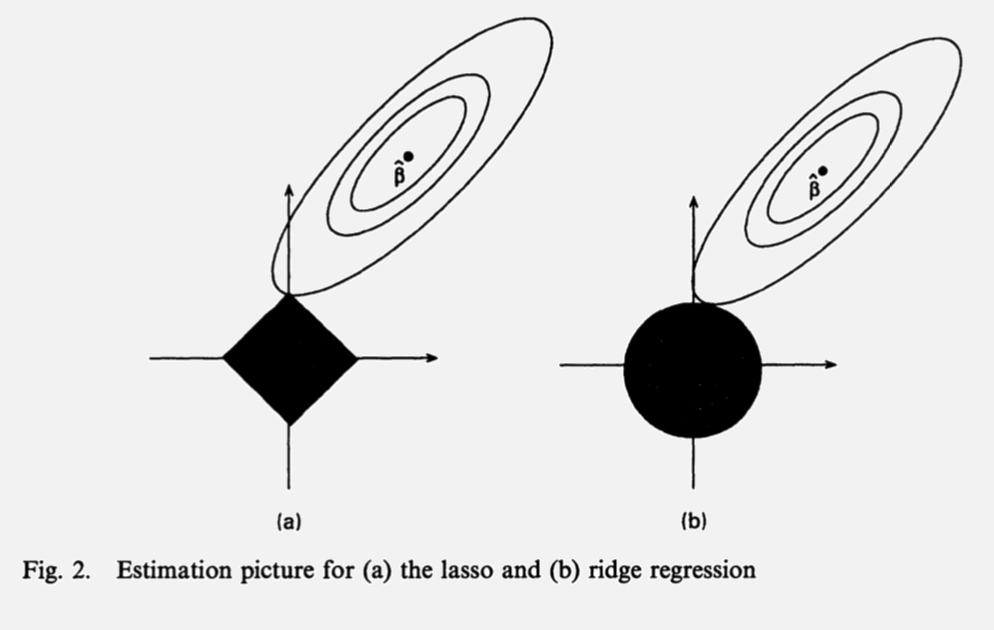
\includegraphics[width=0.67\textwidth, keepaspectratio]{lasso.png}
\caption{Ridge vs LASSO}
\end{figure}
\begin{mdframed}[backgroundcolor=yellow!5] 
\begin{comment}[Can you do both at once?] With \textbf{Elastic Net Regression}, you can. The idea is to use a penalty term that is a convex combination of both $l_1$ and $l_2$ penalty term. Specifically, 
\[
\sum_{i=1}^n(Y_i-X_i\theta_0)^2+\lambda\sum_{k=1}^n\left[\alpha \Vert \theta \Vert_1^2 +(1-\alpha)\Vert \theta \Vert_2^2\right]
\]
If $\lambda=0$ we have an OLS. For $\lambda\neq0$, if $\alpha=1$, we have LASSO, and if $\alpha=0$ we get Ridge. 
\end{comment}
\begin{comment}[Least Angle Regression (LARS)]
The algorithm is as follows
\begin{enumerate}
\item Start with a constant model: For all non-constant covariates, coefficients are 0 and $\lambda=\infty$. 
\item Then, find the covariate that has the largest covariance with the residual. 
\item Change the coefficient for that variable in the same direction as its covariance with the residual ($Y_i- \hat{Y}_i$) until you find a different covariate that has as much covariance with the residuals.  $\lambda$ decrease and $\theta$ is updated along the way.
\item Change the coefficient for the two variables until you find a third variable with the same covariance with the residual. 
\item Stop when all predictors are in the model
\end{enumerate}
When the covariate has the largest covariance with the residual, its angle is smallest. Hence the name LARS. The following figure captures how it works. 
\begin{figure}[H]
\centering
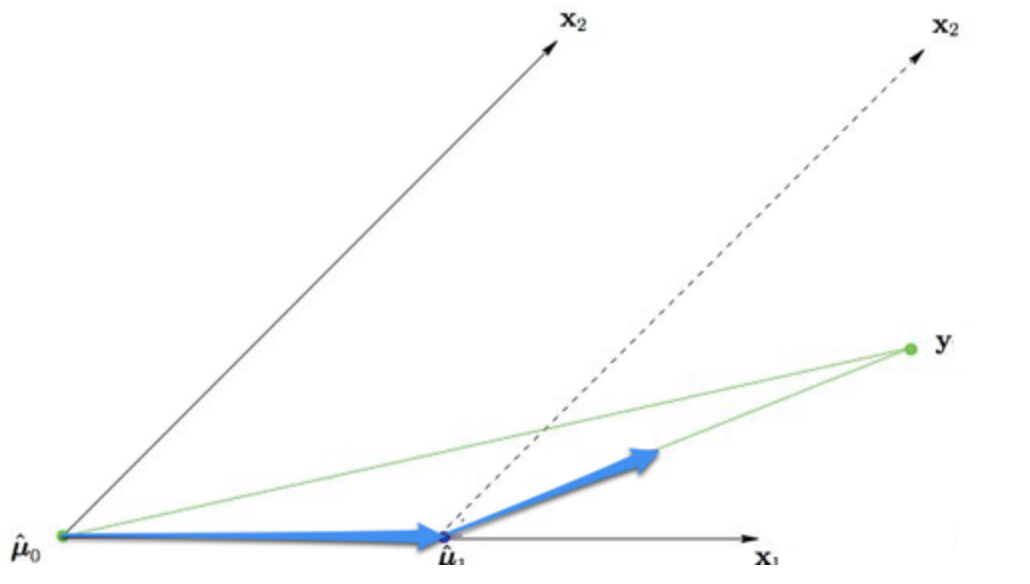
\includegraphics[width=0.67\textwidth, keepaspectratio]{lars.png}
\caption{LARS with two variables}
\end{figure}
\end{comment}
\end{mdframed}
So what is the optimal $\lambda$? It depends on your goal. If your goal is to minimize the prediction error, you can use the following cross-validation methods to come up with one
\begin{itemize}
\item Leave-one-out: Leave one observation out at a time
\item Training vs Test sample: You split the sample into two, build a model given some $\lambda$ and gain prediction error from the test sample. Then, select $\lambda$ minimizing the prediction error there.
\item $K$-fold cross validation:  For $K-1$ blocks, estimate the model given some $\lambda$ and compute the error on the remaining block. Get this for $K$ blocks and compute the average error. Select $\lambda$ minimizing the error. 
\end{itemize}
\subsection{Some Primer on the Consistency of LASSO}
We want to identify what the true model is in a setting with potentially an infinite number of covariates. To do that, we first set a sparsity assumption, where the number of nonzero coefficients is not too large. As a thought experiment, we increase the number of regressors as $n\to\infty$ in order to approximate the true model. To satisfy the assumption, we require that the number of nonzero regressors to rise at a slower rate than $n$. Specifically, $s_n = o\left(\sqrt{\frac{n}{\log p}}\right)$. \par
If we let $\lambda_n = O\left(\sqrt{\frac{\log p}{n}}\right)$ and have $s_n=o\left(\sqrt{\frac{n}{\log p}}\right)$, then we can show that the prediction error goes to 0 and the LASSO estimator is consistent. Or
\[
\frac{1}{n}\sum_i(X_i\hat{\theta}_n-X_i\hat{\theta}_{0n})^2=O_p(\lambda_n^2s_n)
\]
and 
\[
\Vert \hat{\theta}_n-\hat{\theta}_{0n}\Vert_1 = o_p(\lambda_n s_n) = o_p(1)
\]
This comes at the cost of a slightly slower rate of convergence, which is tolerable as long as it is faster than $n^{-1/4}$.
%%%%%%%%%%%%%%%
\end{document}

